\documentclass{article}

\makeatletter
\renewcommand*{\fps@figure}{!htb}
\renewcommand*{\fps@table}{!htb}
\makeatother

\usepackage[a4paper]{geometry}
\usepackage[utf8]{inputenc}
\usepackage[hidelinks]{hyperref}
\usepackage{amsmath, bm}
\usepackage[ruled,vlined]{algorithm2e}
\usepackage[capitalise, nameinlink]{cleveref}
\usepackage{amssymb}
\usepackage{graphicx}
\usepackage{float}
\usepackage{booktabs}
\usepackage[parfill]{parskip}
\usepackage{comment}
\usepackage{subcaption}


\usepackage[sorting=none]{biblatex}
\addbibresource{report_4.bib}

\usepackage{titling}
\setlength{\droptitle}{-3cm}

\title{COMP6247 Final Assignment: Learning Controller}
\author{Wei Chien Teoh (Eugene)\\\bigskip \href{mailto:wct1c16@soton.ac.uk}{wct1c16@soton.ac.uk}}
\date{4 June 2021}

\begin{document}

\maketitle

\section{Introduction}

This report presents the findings and results for the final assignment of COMP6247~\cite{mahesanniranjanCOMP6247202021}. The code implementation is stored in a Github repository \cite{teohEugeneteohCOMP6247ReinforcementOnlineLearning2021}.

\section{Radial Basis Functions}

In this section, we explore the use of Radial Basis Functions (RBF) on Reinforcement and Online Learning problems.

\subsection{Regression}

First, RBF is used to solve a non-linear regression problem. The Airfoil Self-noise Dataset~\cite{UCIMachineLearning} from the UCI repository of machine learning is used as the problem of interest for regression. The dataset consists of samples of aerodynamic and acoustic tests of airfoil blades conducted in a wind tunnel. The features given include:
\begin{enumerate}
    \item Frequency, in Hertz
    \item Angle of attack, in degrees
    \item Chord length, in meters
    \item Free-stream velocity, in metres per second
    \item Suction side displacement thickness, in metres
\end{enumerate}
The output to be predicted is the scaled sound pressure level, in decibels.

% TODO: Mention the RBF parameters, number of centroids, sigmoid etc and explore how it affects the output results
First, we attempt to solve the problem with a linear regression in closed form, $\pmb{W} = (X^T X)^{-1} X^T \pmb{y}$. We then proceed to apply an RBF kernel with Gaussian function. Three approaches were used to solve for the RBF regression parameters:
\begin{itemize}
    \item Closed form, $\pmb{W} = (U^T U)^{-1} U^T \pmb{y}$
    \item Gradient Descent (GD), epochs = 50000
    \item Mini-batch Stochastic Gradient Descent (SGD), batch size = 64, epochs = 10000
\end{itemize}
The Mean Squared Error (MSE) results are shown in \cref{tab:mse-regression}. Linear regression is shown to be insufficient in solving this problem, as the MSE calculated is substantially higher than RBF regression solutions. The RBF closed form solution provided the optimal solution. Both gradient descent methods show convergence of the loss function and also provided similar results, as illustrated in \cref{fig:gd-loss}. However, it is shown that SGD required less number of epochs before convergence. The loss of the gradient descent methods can be further optimised by lowering the learning rate or using adaptive methods or learning rate schedulers.

\begin{table}
    \centering
    \caption{Mean squared error for regression problem.}
    \label{tab:mse-regression}
    \begin{tabular}{lr}
    \toprule
    Model &         MSE \\
    \midrule
    Linear          &  915.288358 \\
    RBF Closed Form &   33.754672 \\
    RBF GD          &   49.234992 \\
    RBF SGD         &   48.822703 \\
    \bottomrule
    \end{tabular}
\end{table}

\begin{figure}
    \centering
    \begin{subfigure}{.49\linewidth}
        \centering
        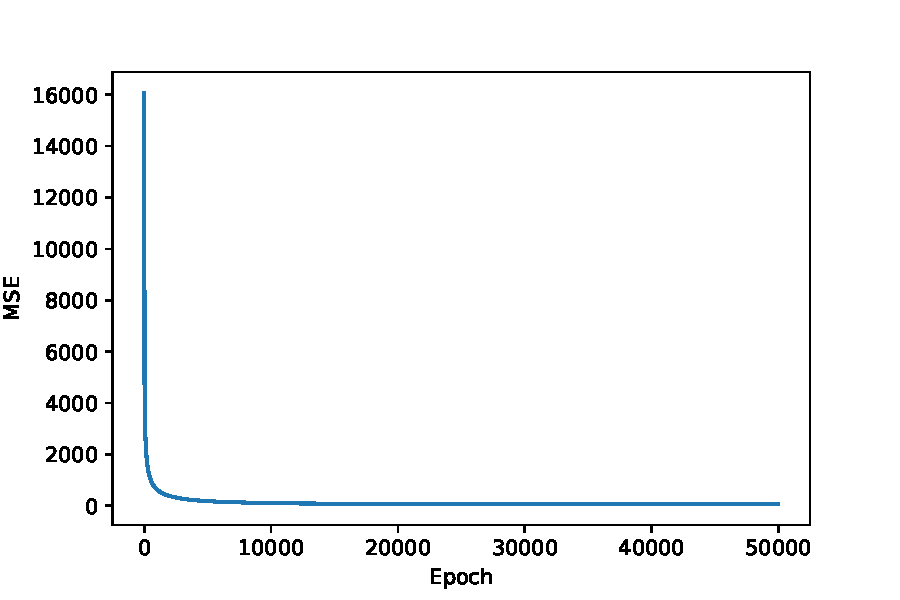
\includegraphics[width=\linewidth]{Figures/gd-loss.pdf}
        \caption{Gradient Descent}
    \end{subfigure}
    \begin{subfigure}{.49\linewidth}
        \centering
        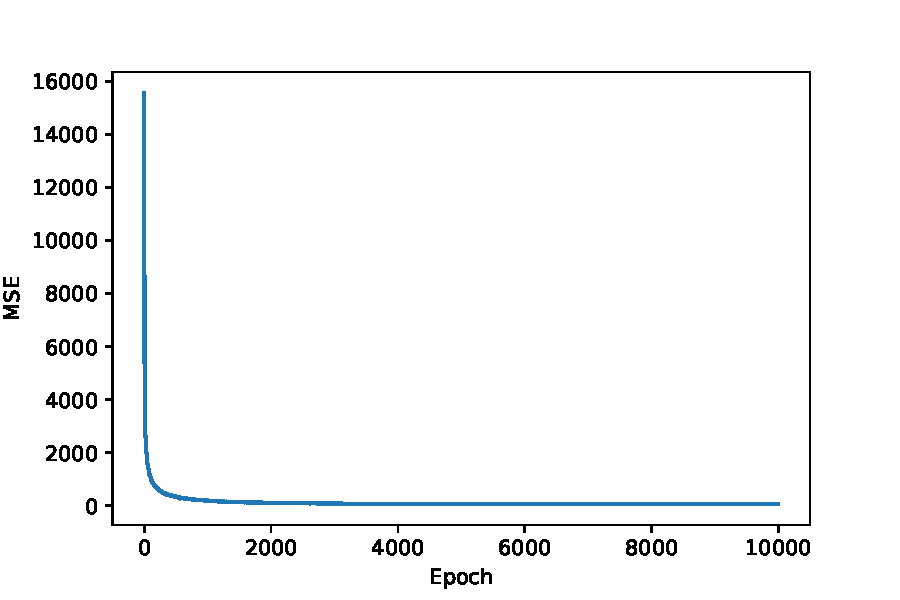
\includegraphics[width=\linewidth]{Figures/sgd-loss.pdf}
        \caption{Stochastic Gradient Descent}
    \end{subfigure}
    \caption{Loss curves for regression using gradient descent approaches.}
    \label{fig:gd-loss}
\end{figure}

\subsection{Mountain Car Learning Controller}


\printbibliography

\end{document}